\section*{Comandos en redes}

\begin{itemize}
    \item \textbf{Ifconfig}: Nos sirve para gestionar, verificar y visualizar las interfaces de red de nuestro sistema, por el momento solo visualizaremos.
    \begin{itemize}
        \item Investiga qué significan los resultados obtenidos y explícalos a grandes rasgos.
    \end{itemize}

    \begin{center}
        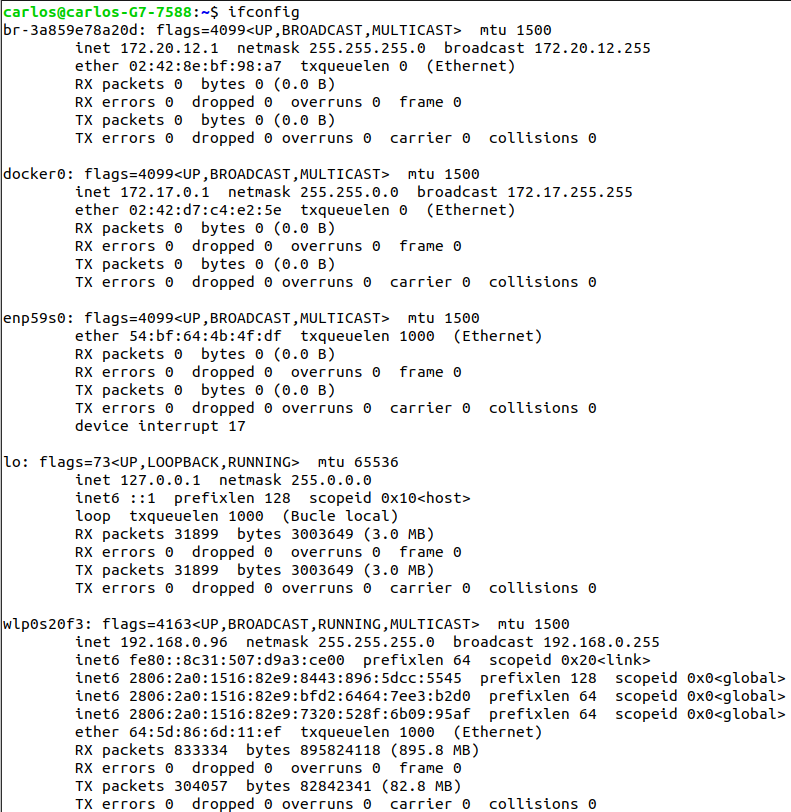
\includegraphics[width=12cm]{IMAGE/ifconfig.png}
    \end{center}
    
    \textbf{br-3a859e78a20d}: Esta es una interfaz de puente creada por Docker. Los puentes permiten a varios contenedores comunicarse en la misma red.
    
    \begin{itemize}
        \item \textbf{flags=4099$<$UP,BROADCAST,MULTICAST$>$}:  La interfaz está activa (UP) y admite difusión (BROADCAST) y multidifusión (MULTICAST).\\
        \item \textbf{mtu 1500}: La Unidad Máxima de Transmisión es de 1500 bytes.\\
        \item \textbf{inet 172.20.12.1}: La dirección IPv4 asignada es 172.20.12.1.\\
        \item \textbf{netmask 255.255.255.0}: La máscara de red es 255.255.255.0.\\
        \item \textbf{broadcast 172.20.12.255}: La dirección de difusión es 172.20.12.255.\\
        \item \textbf{ether 02:42:8e:bf:98}: La dirección MAC es 02:42:8e:bf:98\\
        \item \textbf{TX y RX packets}: Estadísticas de paquetes transmitidos (TX) y recibidos (RX). Actualmente, no ha habido tráfico en esta interfaz.
    \end{itemize}

    \textbf{docker0}: Otra interfaz de puente creada por Docker, utilizada para conectar contenedores Docker a la red.
    
    \begin{itemize}
        \item \textbf{flags=4099$<$UP,BROADCAST,MULTICAST$>$}:  Similar a la interfaz anterior.\\
        \item \textbf{mtu 1500}: La MTU es de 1500 bytes.\\
        \item \textbf{inet 172.17.0.1}: La dirección IPv4 es 172.17.0.1.\\
        \item \textbf{netmask 255.255.255.0}: La máscara de red es 255.255.0.0.\\
        \item \textbf{broadcast 172.20.12.255}: La dirección de difusión es 172.17.255.255.\\
        \item \textbf{ether 02:42:d7:c4:e2:5e}: La dirección MAC es 02:42:d7:c4:e2:5e.\\
        \item \textbf{TX y RX packets}:Estadísticas de tráfico, sin actividad en esta interfaz.
    \end{itemize}

    \textbf{enp59s0}: Interfaz Ethernet física en el sistema.
    
    \begin{itemize}
        \item \textbf{flags=4099$<$UP,BROADCAST,MULTICAST$>$}:  Similar a las interfaces anteriores.\\
        \item \textbf{mtu 1500}: La MTU es de 65536 bytes.\\
        \item \textbf{ether 54:bf:64:4b:4f}: La dirección MAC es 54:bf:64:4b:4f\\
        \item \textbf{TX y RX packets}: Estadísticas de tráfico, sin actividad en esta interfaz.
        \item \textbf{device interrupt 17}: La interrupción del dispositivo es 17, utilizada para manejar las señales del hardware.\\
    \end{itemize}

    \textbf{lo}: Esta es la interfaz de loopback, utilizada para la comunicación interna del sistema.
    
    \begin{itemize}
        \item \textbf{flags=73$<$UP,LOOPBACK,RUNNING$>$}:  Similar a la interfaz anterior.\\
        \item \textbf{mtu 1500}: La MTU es de 65536 bytes.\\
        \item \textbf{inet 127.0.0.1}: La dirección IPv4 de loopback es 127.0.0.1.\\
        \item \textbf{inet6 ::1}: La dirección IPv6 de loopback es ::1.\\
        \item \textbf{RX packets 4405, TX packets 4405}: Estadísticas de paquetes recibidos y transmitidos.\\
        \item \textbf{RX y TX errors}: Sin errores en la transmisión o recepción de paquetes.\\
    \end{itemize}

    \textbf{wlp0s20f3}: Esta es una interfaz inalámbrica en tu sistema.
    
    \begin{itemize}
        \item \textbf{flags=4163$<$UP,BROADCAST,RUNNING,MULTICAST$>$}:  La interfaz está activa, en ejecución, y admite difusión y multidifusión.\\
        \item \textbf{mtu 1500}: La MTU es de 1500 bytes.\\
        \item \textbf{inet 192.168.0.96}: La dirección IPv4 es 192.168.0.96.\\
        \item \textbf{netmask 255.255.255.0}: La máscara de red es 255.255.255.0.\\
        \item \textbf{broadcast 192.168.0.255}: La dirección de difusión es 192.168.0.255\\
        \item \textbf{inet6 fe80::8c31:507:d9a3}: Dirección IPv6 local (enlace local).\\
        \item \textbf{inet6 2806:2a0:1516:82e9:4b0d:1e8c:b841:56ed}: Dirección IPv6 global.\\
        \item \textbf{ether 64:5d:86:6d:11}: La dirección MAC es 64:5d:86:6d:11.\\
        \item \textbf{RX packets 78090, TX packets 41211}: Estadísticas de paquetes recibidos y transmitidos.\\
        \item \textbf{RX y TX errors}: Sin errores en la transmisión o recepción de paquetes.\\
    \end{itemize}
    
    \item \textbf{Ping}: Nos ayuda principalmente a verificar la conectividad entre nuestro sistema y algún otro conectado a una red (por ejemplo, tu computadora y la de tu amigo).
    \begin{itemize}
        \item Haz Ping a \texttt{www.google.com} y a la página de la facultad y mediante una captura muestra el resultado.
        \begin{center}
            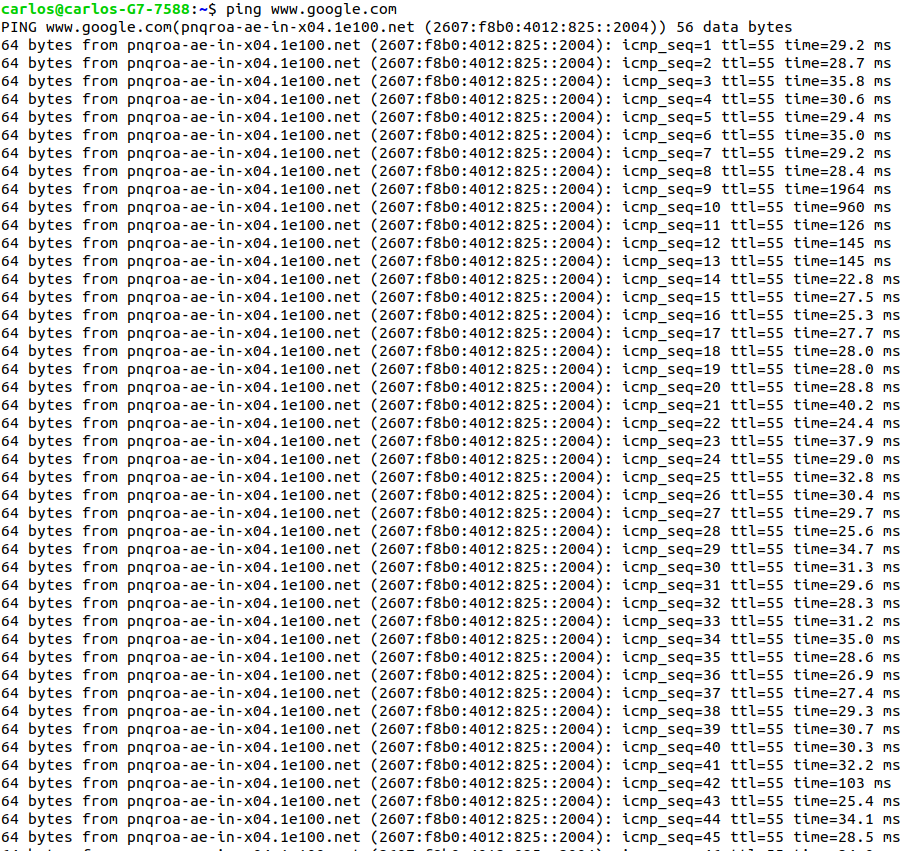
\includegraphics[width=12cm]{IMAGE/google.png}
        \begin{center}
            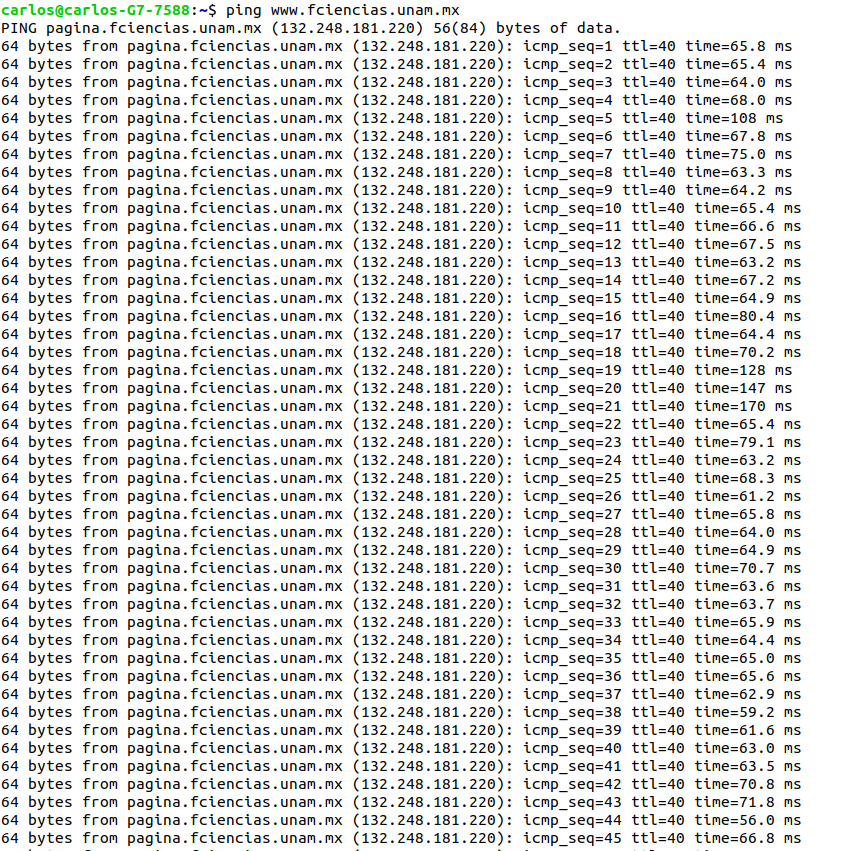
\includegraphics[width=12cm]{IMAGE/fciencias.png}
        \end{center}
    \end{center}
        \item ¿Ves algo diferente?\\

        \textbf{Dirección IP:} Notemos que google una una dirección numérica IPv4, mientras que la pagina de la facultad es una dirección hexadecimal IPv6

        \textbf{Tiempo de Respuesta:} Google presenta mayor variabilidad en sus tiempos de repuesta, dando fluctuaciones de frecuencia, y en la pagina de la facultad obervemos que los timpos de respuesta son mas consistentes sin haber una variación alta.

        También podemos decir que de estos tiempos de respuesta el más estable es el de la facultad, en cambio con los de google dado que los tiempos de respuesta son altos podemos tener problemas de red, o algún otro factor que este influyendo en la conectividad.
        
        \item Usa \texttt{ping -c <número> <ruta>}. ¿Para qué sirve el parámetro \texttt{-c}?\\

        El parámetro $-c$, en el comando ping enviará el número de paquetes que se especificaron y también nos da un resumen de las estadísticas de ping, como podemos observar en la imagen siguiente:
        
        \begin{center}
            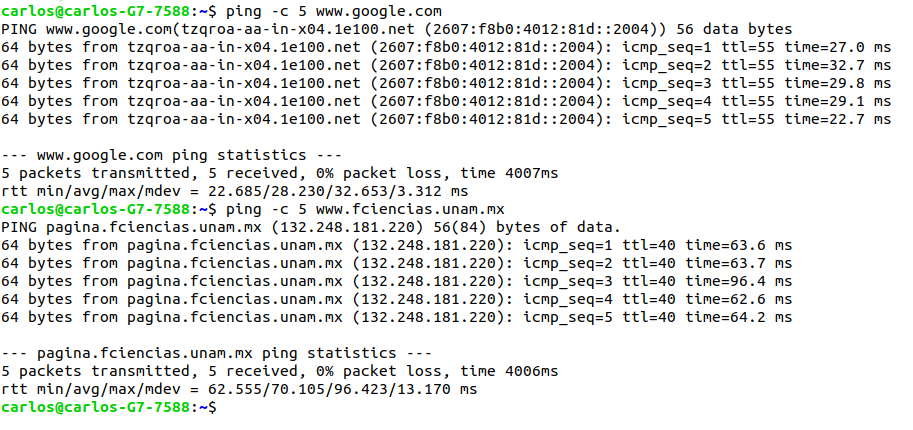
\includegraphics[width=12cm]{IMAGE/ping-c.png}
        \end{center}
        \item Extra: Haz Ping a la computadora de algún compañero de tu equipo y muestra el resultado.

        \begin{center}
            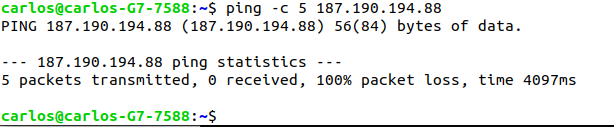
\includegraphics[width=12cm]{IMAGE/ping-computadora.png}
        \end{center}
    \end{itemize}

    \item \textbf{Traceroute}: Es un poco similar a Ping, pero lo que hace es rastrear la ruta que sigue un paquete de datos hasta un destino específico.

        El objetivo principal de esta herramienta es conocer el camino que recorre un paquete a través de nuestra red.
         Este comando de red nos permitirá saber por dónde pasa el paquete (máquinas, switches, routers) y 
         comprobar que nuestra red funciona correctamente. Si detecta cualquier problema, nos va a permitir tener 
         una idea aproximada acerca de dónde se encuentra el fallo. \cite{Pandora2024}

    \begin{itemize}
        \item Realiza las mismas actividades que Ping pero ahora con \texttt{traceroute}.
        
        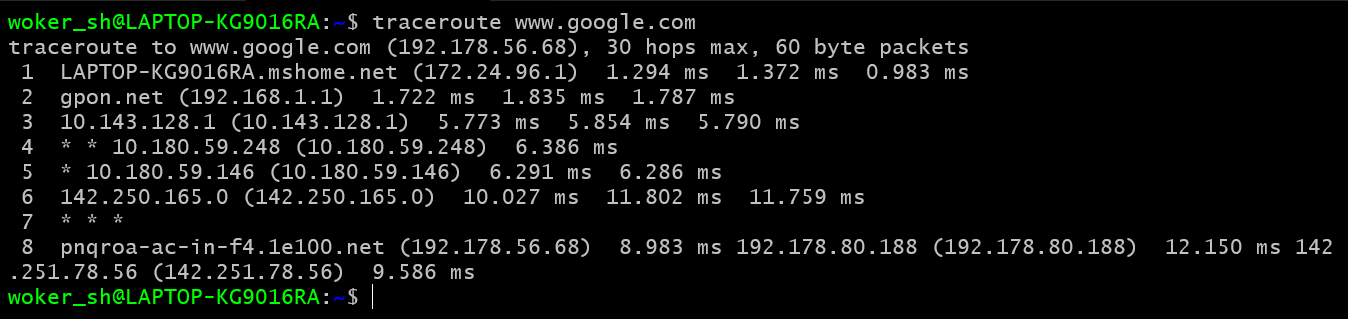
\includegraphics[scale = .3]{IMAGE/Ejercicio2/T01.png}

        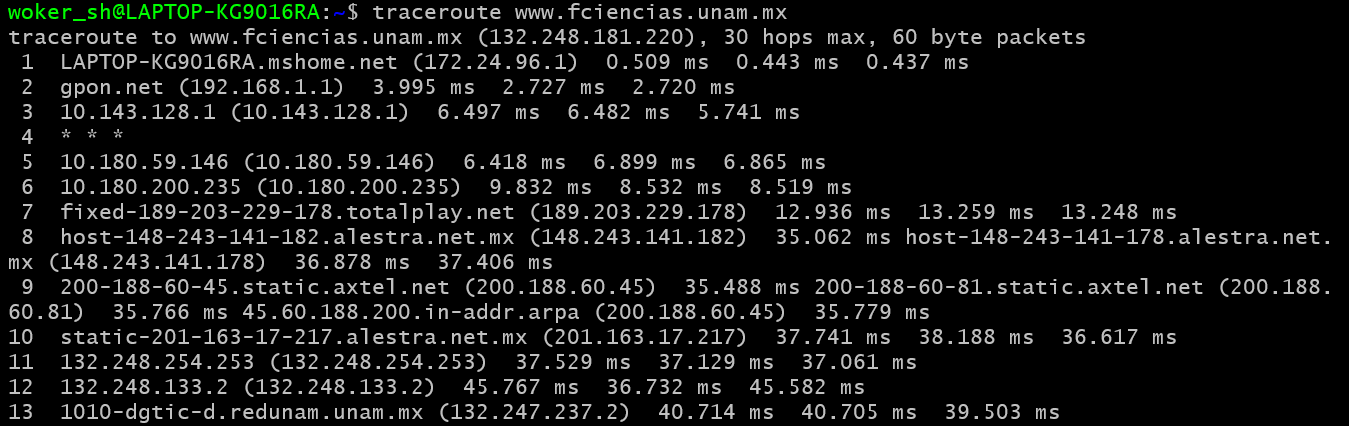
\includegraphics[scale = .3]{IMAGE/Ejercicio2/T02.png}
        
        \begin{itemize}
            \item ¿vez algo diferente?
            La pagiana de google muestra la ruta desde mi lap pasando por varirios enrutadores hasta uno 
            de los servidores de google mientras que la pagina de la facultad muestra una ruta con diferentes 
            rutas en el país finalizando en una que le pertenece a la UNAM. Para google algunos saltos no 
            estan señalados pero para la pagina de Ciencias si se muestran más múltiples redes locales.
        \end{itemize}


        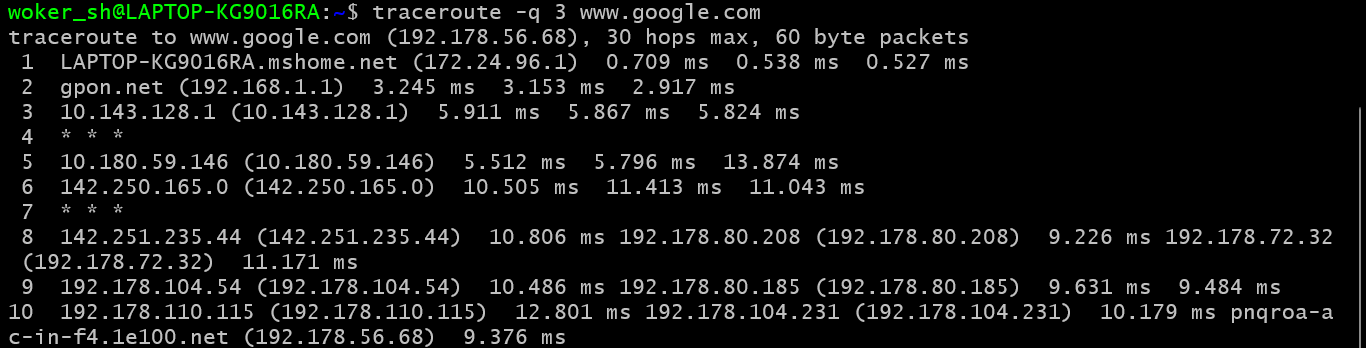
\includegraphics[scale = .3]{IMAGE/Ejercicio2/T03.png}
        \begin{itemize}
            \item \texttt{traceroute -q 3 www.google.com}
            
            El uso de \texttt{traceroute} con opción para múltiples paquetes a diferencia de \texttt{ping} se
            usa \texttt{-q} para especificar el número de consultas en cada salto, en la captura se 
            muestran los tiempos de respuesta para los 3 paquetes enviados a cada salto e indica si esque  
            no se recibieron respuestas en algunos saltos.
        \end{itemize}
    \end{itemize}

    \item \textbf{Netstat}: Este comando nos permite visualizar qué puertos están abiertos, lo cual 
    será muy útil si queremos verificar conexiones. Lista estándar de todas las conexiones activas \cite*{IONOS2022}

    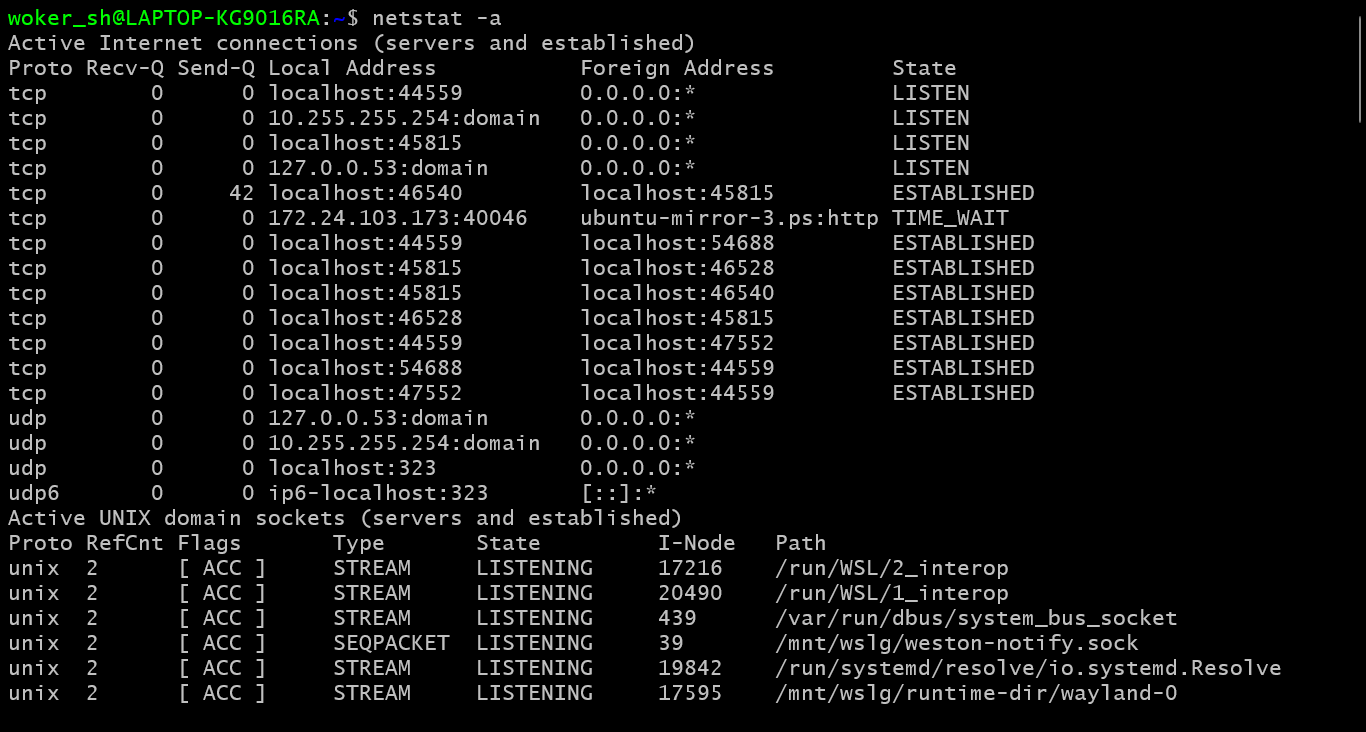
\includegraphics[scale = .3]{IMAGE/Ejercicio2/T04.png}

    \begin{itemize}        

        \item ¿Qué puedes observar?
        \item ¿Qué nos indica cada sección?
        
        \begin{itemize}
            \item Proto: Indica el protocolo de red utilizado (TCP o UDP).
            \item Recv-Q: Muestra la cantidad de datos que han llegado a la cola de recepción pero aún no se han leído por el proceso.
            \item Send-Q: Muestra la cantidad de datos que están en la cola de envío, esperando ser enviados.
            \item Local Address: La dirección IP local y el puerto en el que el proceso está escuchando o conectado.
            \item Foreign Address: La dirección IP y el puerto remoto con el que el proceso está conectado.
            \item State: El estado de la conexión (solo para TCP).
        \end{itemize}

        \begin{itemize}
            \item TCP LISTEN: Puertos que están esperando nuevas conexiones.
            \item TCP ESTABLISHED: Conexiones activas entre el puerto local y un puerto remoto.
            \item TCP TIME WAIT: La conexión ha sido cerrada, pero está en espera de que todos los datos se transmitan correctamente.
            \item UDP: Puertos en los que los servicios están listos para recibir datagramas.
            \item UDP6: Puertos en IPv6 esperando datagramas.
        \end{itemize}

    \end{itemize}

    \item Investiga 3 comandos más que consideres que se usan en redes (no importa si requieren instalación adicional como \texttt{speedtest}) y menciona qué hace cada uno.
    
    \begin{itemize}
        \item comando \texttt{dig} \cite*{ComandDIG}
        
        En su forma más simple, la sintaxis del comando Dig se verá así:
        \begin{center}
            \texttt{dig [servidor] [nombre] [tipo]}
        \end{center}
        
        \begin{itemize}
            \item[] servidor: la dirección IP o el hostname del nombre del servidor a consultar.
            
            Si el argumento del servidor es el hostname, dig resuelve el hostname antes de continuar con la consulta.            

            \item[] nombre: el nombre del registro de recursos que se debe buscar.
            \item[] tipo: el tipo de consulta solicitada por dig. Por ejemplo, puede ser un registro A, 
            un registro MX, un registro SOA o cualquier otro tipo. De forma predeterminada, \texttt{dig} realiza 
            una búsqueda de un registro A si no se especifica ningún argumento de tipo.
        \end{itemize}

        \item comando \texttt{arp} \cite*{IONOSARP}
        
        El Address Resolution Protocol es un protocolo estándar que se puede utilizar en cualquier plataforma y que, 
        como tal, se ocupa de la asignación de direcciones MAC en un segundo plano independientemente del sistema, 
        ya sea Linux, Windows o macOS.\\

        El comando \texttt{arp –a} funciona en cualquier sistema. Al introducirlo aparece una lista de combinaciones
        de direcciones para todas las interfaces de red que utilizan ARP. ¿Cómo funciona? A la hora de 
        asignar direcciones por medio del Address Resolution Protocol hay que distinguir si la dirección IP 
        del host de destino se encuentra en la misma red local o en otra subred. Así, en caso de asignar una 
        dirección MAC a una determinada dirección IP, antes de nada se lleva a cabo una revisión de la 
        máscara de subred. Si la IP se encuentra en la red local, el primer paso es controlar si ya existe 
        una entrada para ella en la caché del ARP.


        \item comando \texttt{ncat} \cite*{IONOSNAT}
        
        Netcat es una herramienta de línea de comandos que sirve para escribir y leer datos en la red. Para 
        la transmisión de datos, Netcat usa los protocolos de red TCP/IP y UDP. La herramienta proviene 
        originalmente del mundo de Unix.

        La sintaxis de Netcat consiste en dos componentes fundamentales: el comando básico “nc”, siempre idéntico, seguido por varias “opciones”. El comando básico direcciona al archivo de programa nc.exe, mientras que las opciones determinan el rango concreto de funciones de la versión de Netcat, por lo que varían dependiendo del sistema operativo y de la versión de Netcat utilizada.

        \begin{table}[h!]
            \centering
            \begin{tabular}{|l|l|}
            \hline
            \textbf{Opciones} & \textbf{Descripción} \\ \hline
            -4 & Fuerza el uso de IPv4 (GNU Netcat) \\ \hline
            -6 & Fuerza el uso de IPv6 (GNU Netcat) \\ \hline
            -d & Elimina Netcat de la consola  \\ \hline
            -D & Habilita la opción de depurar los sockets (GNU Netcat) \\ \hline
            -h (display help) & Muestra la ayuda  \\ \hline
            \end{tabular}
            \caption{Opciones de GNU Netcat}
            \label{tab:netcat_options}
            \end{table}            
    \end{itemize}
\end{itemize}   
